\documentclass[journal]{IEEEtai}

\usepackage[colorlinks,urlcolor=blue,linkcolor=blue,citecolor=blue]{hyperref}

\usepackage{color,array}

\usepackage{graphicx}

\usepackage{listings}

%% \jvol{XX}
%% \jnum{XX}
%% \paper{1234567}
%% \pubyear{2020}
%% \publisheddate{xxxx 00, 0000}
%% \currentdate{xxxx 00, 0000}
%% \doiinfo{TQE.2020.Doi Number}

\newtheorem{theorem}{Theorem}
\newtheorem{lemma}{Lemma}
\setcounter{page}{1}
%% \setcounter{secnumdepth}{0}


\begin{document}


\title{Exploring CNN architectures and evolving CNN agents to learn from each other} 


\author{Alex Lamarche, Undergraduate at Rochester Institute of Technology, Software Engineering}

\markboth{EEEE 547/647 AI EXPLORATIONS, FALL 2021 - SEMESTER PROJECT, November 2021}
{Alex L. Author \MakeLowercase{\textit{et al.}}: Bare Demo of IEEEtai.cls for IEEE Journals of IEEE Transactions on Artificial Intelligence}

\maketitle

\begin{abstract}
A CNN uses convolutional steps to extract abstract features from an image. These features are fed into a fully connected neural network to classify and image based on what features were present. Since a CNN uses training data to learn, backpropagation is necessary. Each layer of the convolutional step needs to compute the gradient of the image features. Since, the gradient must be computed at each node, a modular approach eliminates the processes of calculating the entire loss gradient at once. With that being said, a CNN reduces the input space so much so, that the classifier will be processing an entire image over the span of a few parameters and additionally across a single chained gradient and loss. Since human neural networks don’t rely on the entire brain to recognize images – just sub regions – it would make sense to split the learning process across multiple convolutional agents which each analyze different portions on an image and calculate their own respective gradients. These agents can then conclude by way of voting, which image is presented. 
\end{abstract}

\begin{IEEEkeywords}
genes, CNN, architecture
\end{IEEEkeywords}

\section{Introduction}

\IEEEPARstart{A}{n} important theory as to how our brains function in relation to neural networks relates back to the book A Thousand Brains: A New Theory of Intelligence, by Jeff Hawkins [1,2]. Our brains are comprised of thousands of sub regions that tackle problems and make decisions every day. These regions will take on the problems at different levels of abstraction and pool together to vote on what to do next. I plan to take this basic understanding of the theory and apply it to train a population of agents equipped with convolutional neural networks. Each network shall focus on different areas and features of an input image. During training, agents will swap, modify, and delete, layers and neurons when interacting with another agent. At the end of each learning cycle, two agents, one fit and another not, will reproduce and exchange network information. The “healthy” network will pass genes  (layers and nodes) onto their offspring. Creating a new potentially smarter generation. When it comes time for classification, these agents will pool together their predictions and come to a common vote as to what is being viewed. An example: two convolutional agents inspect an image at different down sampling rates or dilations. Each network is inspecting a relatively similar image, but each use a different feature extraction approach. This ensures that the agents come to different conclusions at different times on different data – even though they are both looking at the same image. When it comes time to validate and vote on a classification, the closest agent to the desired goal is rewarded and the “genes” or parameters that succeeded are exchanged between not so successful agents. This process can be called reproduction and can generate a new agent which performs and learns by its influence on the previous generation.\\ \\
State of the art networks train on networks that have variable parameter space and layer depth. This is what distinguishes networks from each other. I propose that this new approach will leverage multiple agent perspectives and levels of abstraction, coupled with a voting system (or voting layer) that combines the votes and errors such that each new generation of agents learns and trains at the same time. New generations will come and go during the training process. The final network is comprised multiple agents voting on different abstractions of an image. These final trained agents are the regions of the brain that are independent of each other in terms of direction connection, yet still affect the outcome of a classification.

\subsection{Background and Benchmarks}

To simplify, the most important benchmarks for this model will focus on layer depth (l), parameter count (p), average speed in milliseconds of forward and backward passes (f,b), and overall accuracy of prediction (a). Once metrics are gathered for different agent populations, only then can I compare current popular networks performances to mine. Current benchmarks can be seen to have milliseocond pass time in forward and backward direction [2,3]


\subsection{Approach}
I will construct a CNN and classifier from scratch using python and a few helper libraries for linear transformations and graphical plotting. I ensure that each layer is modular that way networks can be constructed on the fly, can be manipulated, and can differ and sizes. For now, a simple (Conv, Pool, ReLU)x3  network is constructed using the software architecture developed. Convolutional objects take in an input image as their first parameter and any number of layer filters, pools, and activations as the remainder of the parameters. Filters/Kernels, pooling layers, and activation layers are all referred to as genes. These genes each follow a loose interface which implements a forward() function and a backward() function. The forward pass is responsible for feature extraction and passing convolved / modified layers to the next. The backward() function is responsible for calculating the gradient. Filters (kernel), otherwise known as convolutions, and activation functions are the only layers that need complex derivations for their gradients. Other layers like max pooling only need to pass their maximum value back up the network in an attempt to rescale the image upward. 

\clearpage
\begin{lstlisting}
conv = c.Convolutional(
    input=image_in,
    l1=c.Filter(matrix=[
        [0, -1, 0],
        [-1, 5, -1],
        [0, -1, 0]
    ]),
    l2=c.MaxPool(size=2),
    l3=c.ReLU()
)
out = conv.start()

\end{lstlisting}

On start() each layer undergoes its forward pass. Once the forward passes are complete, the function will calculate the loss compared to the actual value. This loss should then be propagated throughout the network by means of the backwards pass function. Here is a high-level implementation of the forward and backward pass functions:

\begin{lstlisting}
class Filter:
    def __init__(self, matrix):
        self.matrix = matrix
        self.size = len(matrix)

    def forward(self, img):
        pass
    def backward(self,dL):
        pass
\end{lstlisting}

here the filter class is a main executer of the convolution. Its forward function slides a matrix overtop the input image and amplifies and modifies features to be passed down the network stream. The backward function gets called after the start() function completed all forward passes for one input sample. dL variable in the backwards pass is the previous layers derivative. Or downstream loss. This is the gradient from the previous layer. Each layer will receive an upstream gradient from the previous layer and calculate a new downstream gradient which will go to the next layer. This chaining of gradients is called the chain rule. Instead of calculating our networks entire gradient in one go, we can let the network chain partial derivatives as it propagates. This network demonstrates modularity.

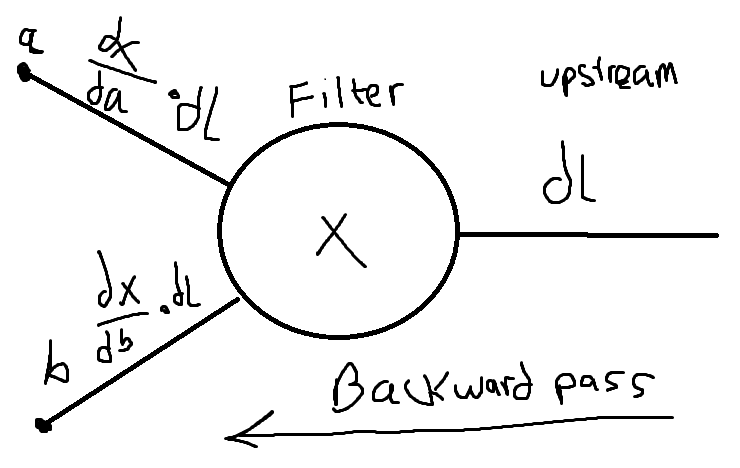
\includegraphics[scale=.4]{modularity.png}

\subsection{Unfinished Work}
I need to work out the derivatives for the Filter pass. And the average pooling gradient. Once done, I can start to work on the fully connected layer that attaches to the tail end of the convolutional network. This Fully Connected network will be similar to the convolutional one, except that each layer connects to each of the nodes in the next layer. The final layer is a 10-parameter solution vector. This vector will produce a loss value which can then initiate the gradient descent process.
Once this is done, I can start to run the CNN on MNIST written digits. Once I minimize the cost and predict digits with fairly high accuracy, I will then start training agents in parallel; exchanging genes and comparing metrics between experiments.

\section*{References and Footnotes}

\subsection{References}
[1] Hole, K. J., \&amp; Ahmad, S. (2021, July 20). A thousand brains: Toward biologically constrained ai. SN Applied Sciences. Retrieved November 22, 2021, from https://link.springer.com/article/10.1007/s42452-021-04715-0. 

[2] https://github.com/jcjohnson/cnn-benchmarks
 
[3] https://paperswithcode.com/sota/image-classification-on-mnist


\end{document}
